\documentclass[12pt,a4paper]{article}
\usepackage[utf8]{inputenc}
\usepackage[english]{babel}
\usepackage[T1]{fontenc}
\usepackage{amsmath}
\usepackage{amsfonts}
\usepackage{amssymb}
\usepackage{lmodern}
\usepackage{graphicx}
\usepackage{parskip}
\usepackage{moreverb}
\usepackage{float}
\usepackage{placeins}

%% Bibliography %%
\usepackage[notlof]{tocbibind}

%% Table %%
\usepackage[table]{xcolor}
\usepackage{array}
\usepackage[hidelinks]{hyperref}

\usepackage{subcaption}
\usepackage{parskip}
\usepackage[top=2.5cm, bottom=2.5cm, left=2.5cm, right=2.5cm]{geometry}

%% Header
\usepackage{fancyhdr}
\setlength{\headheight}{15pt}
\pagestyle{fancy}
\fancyhf{}
\rhead{\fancyplain{}{\rightmark }}
\lfoot{\textit{INFO0948: Introduction to Intelligent Robotics}}
\rfoot{\thepage}
\renewcommand{\footrulewidth}{0.5pt}

%% Color %%
\usepackage{color}
\definecolor{mygrey}{rgb}{0.9, 0.9, 0.9}
\definecolor{mygreen}{rgb}{0, 0.6, 0}
\definecolor{myblue}{rgb}{0, 0, 0.6}

%% Listings %%
\usepackage{listings}
\lstset{
backgroundcolor = \color{mygrey},
language = Python,
frame = single,
basicstyle = \footnotesize,
keywordstyle = \color{myblue},
commentstyle=\color{mygreen},
numbers = left,
numberstyle = \normalsize,
numbersep = 4pt,
}
%%%%%%%%%

%%%%%%%%%%% TITLEPAGE %%%%%%%%%%%%

\author{EWBANK Tom \\S102705\\Master in Computer Science Engineering (1st year)\\-\\MOMBAERTS Laurent\\S072920\\Master in Biomedical Engineering (2nd year)}
\title{INFO0948: Introduction to Intelligent Robotics}
\date{June 2015}
\begin{document}
\makeatletter
  \begin{titlepage}
  \centering
      {\large \textsc{University of Liège}}\\
      \textsc{Faculty of applied sciences}\\
      \vspace*{0.5cm}
      \hrule
    \vfill    
    	{\LARGE \textbf{Project report:\\}}
    	{\LARGE Programming a youBot in a simulator}
    \vfill
      
\includegraphics[width=10cm]{logo_ulg.png}
     \vfill
      {\large \@title \\ \  \\ \large \@date}
      
    \vfill
    \hrule
        {\large \@author} \\
  \end{titlepage}
\makeatother
%%%%%%%%%%%%%%%%%%%%%%

\tableofcontents
\newpage

\section{Overview}

\paragraph{}
In this work, we implemented a program that allows the 
youBot to move cylindrical and box-shaped objects from a table to their 
appropriate storing locations. 

\paragraph{}
The youBot first explore the environment where it 
evolves and builds a map, knowing its accurate 
location. During the process of building this map, the 
youBot is able to locate circular obstacles of a fixed 
size. When it recognizes such an obstacle, the youBot 
has two choice: either it's a table, either it's a 
basket. There are only two tables and they are visible 
with the Hokuyo sensor from the youBot's starting 
position, no other cylindrical objects are within sight 
of the Hokuyo from the youBot's starting position, so 
it can directly record their location. Each basket is 
associated with a different landmark object placed next 
to itself, and the youBot is able to identify these 
objects. The youBot can thus keep in memory the location 
of each basket and the object associated with them.


\paragraph{}
When the entire map has been explored, the job of the 
youBot is to grab objects from the tables and put them 
into the appropriate baskets. The storing location of 
the objects are determined based on their shape, their 
color, and the instructions that are supplied. For 
example, the youBot knows that a red cylinder should be 
placed in a basket next to a pumpkin. 

\paragraph{}
Our implementation only allows the youBot to grab 
objects that are at the egde of the table, stand 
upright, and are well separated from each other. This configuration is present on the table at the right of the youBot, when it is at its starting position (see figure \ref{youbotStart}). The youBot will thus try to move the objects that are on that table only. The arm of the youBot is moved most of the time using V-REP inverse kinematics.

\paragraph{}
We've thus adressed the milestones A1, B1, C2 and D2 of the project statement\cite{trs}.

\begin{figure}[h]
	\centering
		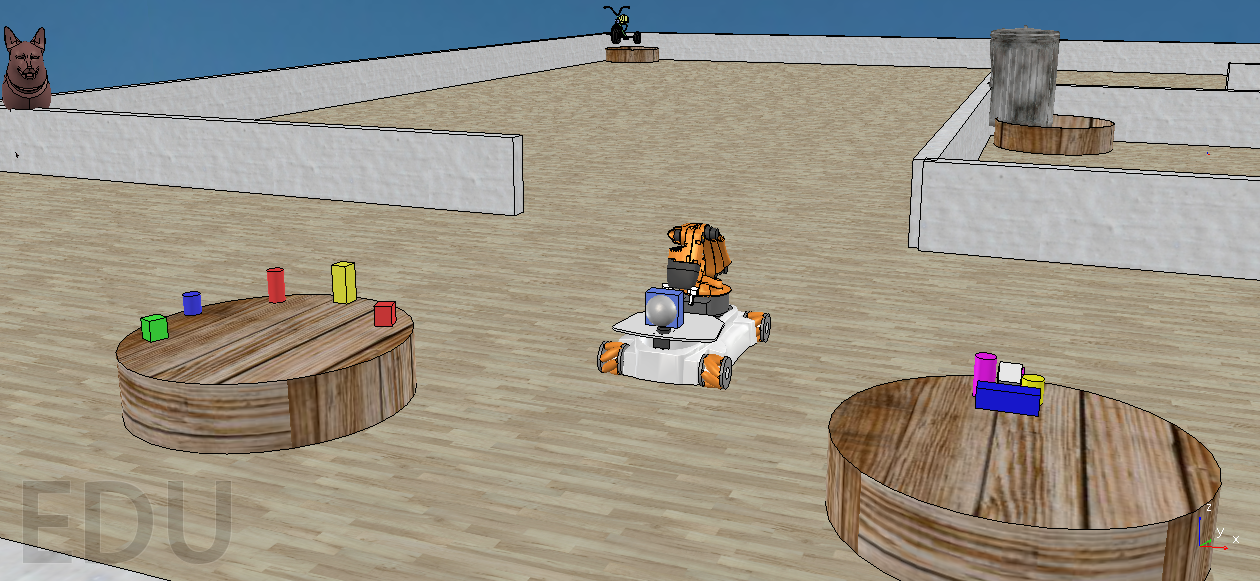
\includegraphics[width=1.00\textwidth]{starting_position.png}
	\caption{Example of a youBot starting position and its environment}
	\label{youbotStart}
\end{figure}

\FloatBarrier

\section{Implemented solutions}

\subsection{Map exploration}
\paragraph{}
The youBot stores a matrix representing the the map. The elements of this matrix can have three different values. One value represent the fact that a cell of the map hasn't been explored yet, another means that it has been, and the last one implies the presence of an obstacle in the cell. During its exploration, the youBot can thus gather the data supplied by its Hokuyo sensors and update the values of this matrix. These data comes in the form of a series of points, in the reference frame of the youBot, that indicate where the range of the sensor stopped, and if it encountered an obstacle or not. Because the youBot knows its accurate position in the map, it can simply transpose these coordinates into the reference frame of the map, and then update the matrix accordingly, including of course all the points in the area swept by the sensor, not only those delimiting its range.   

\paragraph{} 
Now that we've explained how the youBot represents and updates its map, it remains to describe how the youBot will achieve to explore its environment entirely. Our exploration algorithm is the following:

\begin{enumerate}
\item The youBot rotates around itself in order to get a $360^{\circ}$ view of the map

\item The youBot selects the nearest unexplored point and establishes the trajectory to reach it

\item The youBot follows the trajectory, updates the map at the same time and makes sure that it's not running into an obstacle that wasn't yet acknowledged when the trajectory was established, otherwise, it goes back to step 2.

\item When the youBot reached his goal, \\if there is still unexplored points on the map: it goes back to step 2 \\else: the hole map has been explored.

\end{enumerate}



\subsection{Trajectories}

\paragraph{}
The trajectories of the youBot are calculated thanks to the (partial) map and the distance transform function from Peter Corke's robotics toolbox\cite{CorkeRTB}. 

\subsection{Locating an identifying baskets}

\paragraph{}


\subsection{Moving objects}

\paragraph{} 




\clearpage
\begin{thebibliography}{9}

\bibitem{trs}
Detry, Renaud. "Project definition" \textit{TRS: An Open-source Recipe for Teaching/Learning Robotics with a Simulator}. \\
\url{http://ulgrobotics.github.io/trs/project.html}

\bibitem{CorkeBook}
Corke, Peter. \textit{Robotics, Vision \& Control.} 2011.\\
\url{http://www.petercorke.com/RVC/}

\bibitem{CorkeRTB}
Corke, Peter. \textit{Robotics Toolbox for MATLAB}. Release 9. \\
\url{http://www.petercorke.com/Robotics_Toolbox.html}




\end{thebibliography}

\end{document}